%\documentclass{report}
%\usepackage[T1]{fontenc}
%\usepackage[utf8]{inputenc}
%\usepackage[francais]{babel}
%\usepackage{amsmath}
%\usepackage{graphicx}
%\graphicspath{{Figures/}}
%\usepackage[backend=biber,style=authoryear,bibencoding=utf8]{biblatex}
%\usepackage[colorlinks,linkcolor=blue]{hyperref}
%
%
%\addbibresource{biblio.bib}
%
%\begin{document}
\chapter{La cellule et son environnement mécanique}


La cellule est l'unité de base des êtres vivants. Elle peut puiser de l'énergie du milieu extérieur afin de se maintenir dans un état organisé et de se reproduire pour donner naissance à d'autres cellules par la division cellulaire. 

Une cellule est séparée du milieu extérieur par une membrane. Elle contient son code génétique sous la forme d'ADN, elle le duplique et le transmet lors de ses divisions. 

Les cellules sont séparées en deux grands groupes en fonction de l'état de leur ADN : les procaryotes et les eucaryotes. 
L'ADN des procaryotes est libre dans la cellule, il est souvent constitué d'un seul chromosome circulaire. 
Au contraire, l'ADN des eucaryotes est confiné dans un compartiment spécial, le noyau. 

Chez les eucaryotes comme chez les procaryotes, il existe des organismes vivants pouvant être composés d'une ou de plusieurs cellules (\cite{grosberg_evolution_2007}).
Les plus grands organismes, comme les plantes ou les animaux, peuvent être composées d'un très grand nombre de cellules (de l'ordre de $10^{14}$) qui possèdent le même génome mais ont des phénotypes très divers. 

\section{Organisation de la cellule eucaryote}
\begin{figure}[h!]
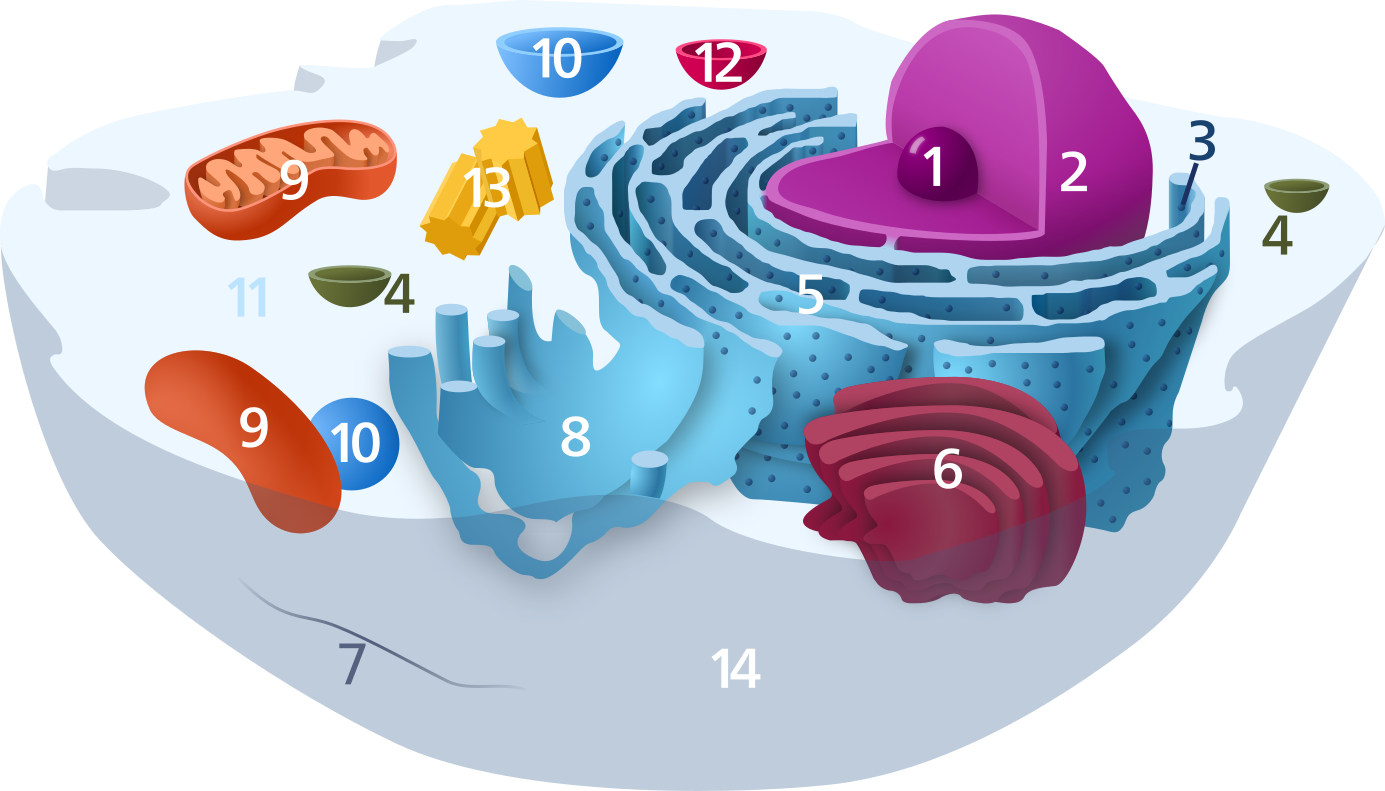
\includegraphics[scale=0.2]{Animal_Cell.png}
\caption{La cellule eucaryote. 
1. Nucléole
2. Noyau
3. Ribosome
4. Vésicule
5. Réticulum endoplasmique rugueux
6. Appareil de Golgi
7. Cytosquelette
8. Réticulum endoplasmique lisse
9. Mitochondrie
10. Vacuole (cellule végétale uniquement)
11. Cytosol
12. Lysosome
13. Centrosome
14. Membrane Plasmique
Figure par Kelvinsong (CC0)}
\end{figure}


Les cellules eucaryotes sont composées de plusieurs compartiments aux fonctions spécifiques à l'intérieur d'une membrane plasmique. Le noyau est le plus gros de ces compartiments, il renferme l'ADN organisé sous la forme de chromosomes et est le lieu de la transcription de l'ADN en ARN. 
Le réticulum endoplasmique rugueux est le siège de la traduction de l'ARN en protéines. 
L'appareil de Golgi est le lieu de transformation finale des protéines. 
Les mitochondries sont les unités de production d'énergie de la cellule : elles produisent l'Adénosine Triphosphate (ATP), qui sera transformée en Adénosine Diphosphate (ADP) en libérant de l'énergie. Les mitochondries seraient d'anciennes bactéries devenues symbiotiques des cellules eucaryotes, elles possèdent leur propre ADN. 

\subsection{L'énergie dans la cellule}

Une cellule vivante est un système très éloigné de l'équilibre thermodynamique. Pour se maintenir en vie, elle utilise donc de l'énergie qu'elle va trouver dans le milieu extérieur. 

À l'intérieur de la cellule, la source d'énergie utilisée dans les réactions enzymatiques est l'hydrolyse de nucléosides triphosphates. 
Il s'agit majoritairement d'Adénosine Triphosphate, qui est hydrolysée en Adénosine Diphosphate et un phosphate inorganique en libérant de l'énergie. 
Les protéines qui utilisent l'ATP comme source d'énergie sont des ATPases. 
C'est le cas par exemple de l'actine lors de sa polymérisation et de la myosine  lors de la contraction musculaire, dont nous ferons une description plus détaillée plus loin. 

Certaines protéines utilisent à la place de l'ATP le Guanosine Triphosphate, fonctionnant de la même manière. 
C'est pas exemple le cas des microtubules ou des petites GTPases comme RhoA, dont nous parlerons également plus loin. 

L'ATP ne peut pas être puisée directement dans le milieu extérieur. Les sources d'énergie des cellules animales sont les glucides simples (comme les sucres) ou complexes (comme l'amidon) et les lipides ou les acides aminés lorsque les autres sources font défaut. 

La cellule animale reçoit principalement son énergie sous forme de glucose par la circulation sanguine. Ce glucose est alors dégradé d'abord dans le cytoplasme, puis en présence de dioxygène dans la mitochondrie. 
Une molécule de glucose permet d'obtenir une trentaine d'ATP. 
Lorsque le dioxygène vient à manquer, par exemple lors d'efforts musculaires intenses, la fermentation permet de produire de l'énergie à partir du glucose en produisant de l'acide lactique. 

\subsection{Le noyau}

Le noyau est l'organite contenant le matériel génétique de la cellule sous la forme d'ADN (à l'exception de l'ADN mitochondrial) . Cependant, bien d'autres molécules que l'ADN sont présentes dans le noyau, et il s'y passe d'autres choses que la transcription ou la duplication de l'ADN. 

\subsubsection{ADN}

\begin{figure}
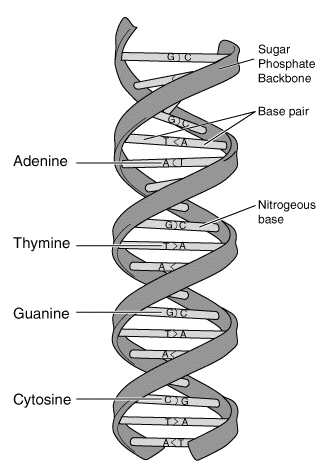
\includegraphics[scale=0.3]{ADN.png}
\caption{Schéma de la structure de l'ADN, par Messer Woland CC-BY-SA-2.5}
\end{figure}

L'ADN est une molécule constituée d'un enchaînement de nucléotides composés d'une base azotée, d'un sucre et d'un groupement phosphate. Il existe quatre bases azotées possibles : Adénine , Thymine, Cytosine, Guanine. Leur enchaînement va être à la base du code génétique.
L'enchaînement des nucléotides forme une double hélice dans laquelle les nucléotides se correspondent en deux paires : Adénine et Thymine, Cytosine et Guanine. 

Le génome des êtres vivants comporte typiquement du million au milliard de paires de base d'ADN. La distance entre deux bases est de 0,34nm. Chez l'homme, on compte environ 3,2 milliards de paires de bases, ce qui correspond à une longueur d'ADN de l'ordre du mètre, qui doit être stockée dans le noyau cellulaire d'un diamètre de 5 à 7 microns. 
On conçoit alors qu'une organisation spécifique de l'ADN dans le noyau soit nécessaire pour faire tenir une molécule aussi grande dans un compartiment aussi étroit. 

\begin{figure}[h!]
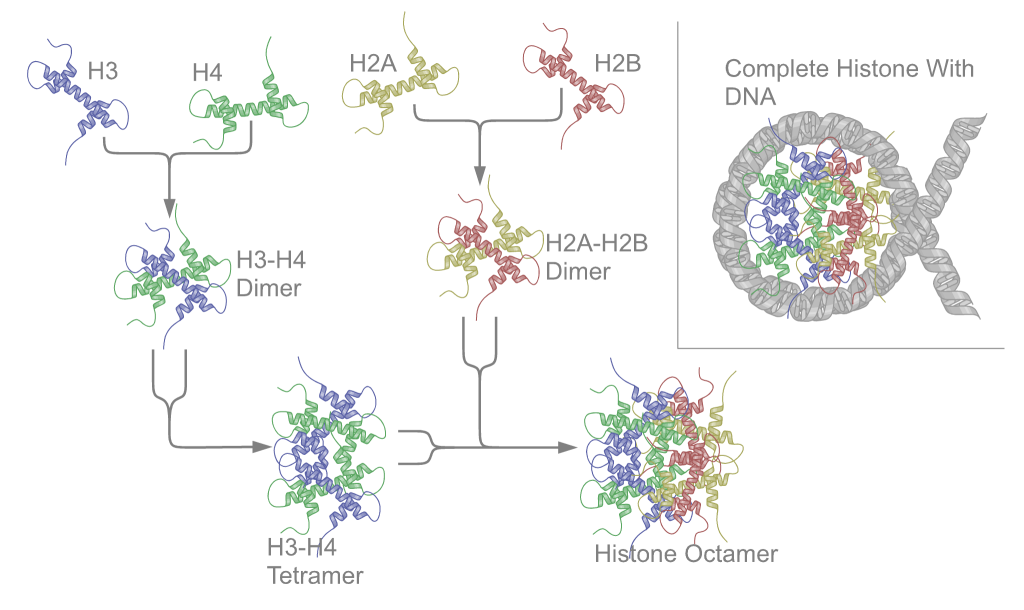
\includegraphics[scale=0.3]{Nucleosome_structure_by_richard_wheeler}
\caption{Enroulement de l'ADN autour d'un complexe d'histones, illustré par Richard Wheeler (CC BY-SA 3.0)}
\end{figure}

L'ADN est enroulé autour de protéines appelées histones comme du fil autour d'une bobine, formant une structure appelée nucléosome. Ces nucléosomes empilés forment une structure bien plus compacte que l'ADN libre, appelée la chromatine. Certains acides aminés qui composent les histones peuvent subir des réactions chimiques comme l'acétylation ou la méthylation, qui ont un rôle dans la régulation de la transcription du génome. L'acétylation des histones peut changer l'état de la chromatine : l'hétérochromatine est la forme compacte où l'ADN ne peut pas être transcrit, l'euchromatine est la forme plus étendue dans laquelle l'ADN est accessible pour la transcription. 

\subsubsection{Transport nucléo-cytoplasmique}
\begin{figure}
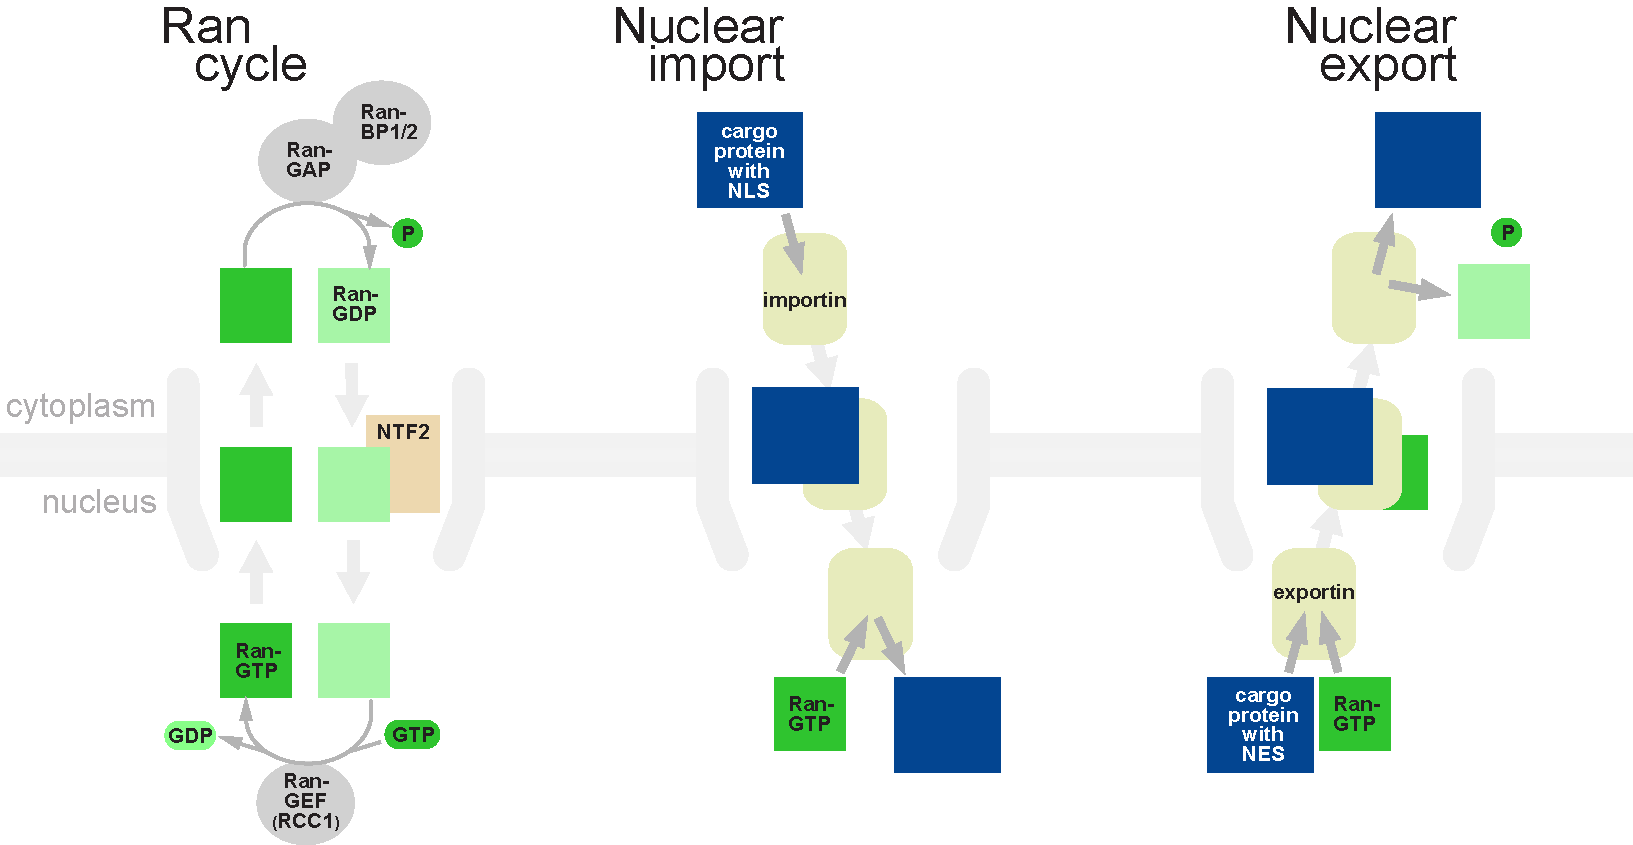
\includegraphics[scale=0.8]{Rancycle_nuclearimport_nuclearexport.png}
\caption{Schéma du transport nucléo-cytoplasmique par les karyophérines.}
\end{figure}
Le noyau est séparé du reste du cytoplasme par une membrane formée de deux bicouches lipidiques. Elle contient des complexes de protéines qui servent de portes d'entrée et de sortie  et qui sont appelées pores nucléaires. Les protéines de taille inférieure à 40 kDa peuvent passer par diffusion passive par les pores nucléaires. 

Les protéines de plus grande taille doivent faire appel à des transporteurs spécifiques pour aller d'un côté de la membrane à l'autre. 
Les importines de lient à la protéine à importer au niveau d'une zone appelée \og Signal de Localisation Nucléaire \fg (NLS). Le couple importine-cargo va diffuser à travers le pore nucléaire. 
Une fois dans le noyau, l'importine va se lier à la RanGTP et se dissocier du cargo, qui est libéré dans le nucléoplasme. L'importine est alors à nouveau exportée du noyau et la GTP hydrolysée en GDP. 
De même, une protéine possédant une séquence d'export nucléaire (NES) sera liée à une exportine-GTP, et le couple diffusera vers le cytoplasme. Une fois dans le cytoplasme, la GTP est hydrolysée en GDP et le cargo relargué. L'exportine revient dans le noyau par diffusion. 

Par exemple, l'actine, bien que de taille 42kDa, à la limite de la diffusion passive, est importée de manière active par l'importine 9 et exportée par l'exportine 6. 

\subsection{La membrane plasmique}

La membrane plasmique sépare le milieu intérieur de la cellule de l'extérieur. Elle est composée d'une bicouche de phospholipides amphiphiles dans laquelle sont enchâssées des protéines transmembranaires qui permettent de réguler les échanges avec le milieu. 

\begin{figure}
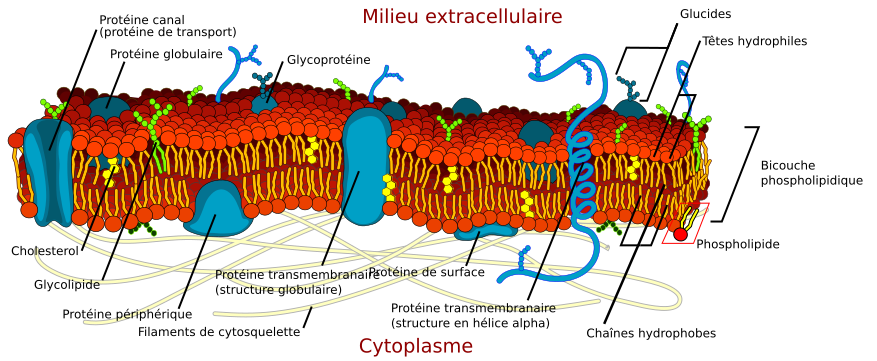
\includegraphics[scale=0.5]{Cell_membrane_detailed_diagram_fr.png}
\caption{Schéma de la membrane plasmique}
\end{figure}
\subsubsection{Transport transmembranaire}
La membrane permet de réguler le passage de molécules d'un côté à l'autre de manière active ou passive. 
 Il existe une très grande variété de transporteurs d'espèces chimiques à travers la membrane. 

Les lipides peuvent passer par diffusion à travers la membrane plasmique, c'est le cas par exemple des hormones stéroïdiennes comme les androgènes ou les \oe strogènes, dont les récepteurs sont à l'intérieur de la cellule et non sur la membrane.

Les ions comme le calcium, le potassium ou le magnésium sont transportés par des canaux spécifiques. Le mouvement des ions permet de polariser la membrane et de faire passer un signal électrique et est essentiel dans le fonctionnement du système nerveux et dans la contraction musculaire. Des canaux spécialisés, les aquaporines, laissent passer l'eau pour moduler la pression osmotique.

Des molécules peuvent également être transportées de l'extérieur vers l'intérieur par l'invagination d'une partie de la membrane en une petite vésicule. Ce phénomène s'appelle l'endocytose. Inversement, des vésicules dans le milieu intracellulaire peuvent fusionner avec la membrane pour émettre leur contenu vers l'extérieur, c'est l'exocytose. Les cellules fabriquant la matrice extra-cellulaire utilisent l'exocytose pour excréter les protéines synthétisées. 

\subsubsection{Signalisation}

La liaison d'un récepteur membranaire à un ligand peut déclencher une activité enzymatique, une ouverture de canaux ioniques ou l'activité des protéines G (dont les petites GTPases). 
La famille des protéines à 7 segments transmembranaires, par exemple, est responsable de la détection des signaux visuels, olfactifs, gustatifs, inflammatoires \dots

\subsubsection{Adhésion}

La plupart des cellules font partie d'un tissu et adhèrent à d'autres cellules voisines et aux protéines de la matrice extra-cellulaire par l'intermédiaire de protéines transmembranaires. 

\paragraph{Interactions cellules-cellules}Les cellules se lient les unes aux autres pour se reconnaître, communiquer et former une structure complète. 

La super famille des immunoglobulines comprend des molécules d'adhésion (IgCAM), souvent spécifiques à un type cellulaire. Elle comprend également les complexes majeurs d'histocompatibilité, qui permettent au système immunitaire de reconnaître les cellules de son propre organisme. 

Les cellules échangent entre elles des espèces chimiques et des signaux électriques. 
Les jonctions communicantes permettent une communication directe entre deux cellules en contact. Les espèces chimiques peuvent passer librement de l'une à l'autre. Cela peut amplifier un signal hormonal, perçu par une cellule et transmis à travers ces jonctions aux voisines qui n'ont pas capté le signal directement. Elles peuvent également servir à transmettre très rapidement un signal électrique. 
Les synapses sont un système très élaboré de communication entre deux cellules par échange d'espèces chimiques (les neurotransmetteurs) par exocytose dans un espace inter-cellulaire réduit. 

Au contraire, les jonctions serrées permettent de créer une étanchéité de part et d'autre d'une monocouche cellulaire. Les cellules épithéliales forment un feuillet continu lié par des jonctions serrées qui maintient la séparation entre le milieu extérieur (la lumière) et le milieu intérieur, par exemple au niveau de la peau, des muqueuses, de l'intérieur du tube digestif\dots

Les cadhérines forment une famille de protéines exprimées partout dans l'organisme à tous les stades de son développement. 
Il existe une trentaine de gènes de cadhérines, et encore plus de protéines exprimées grâce à l'épissage. Ces différentes protéines sont spécifiques selon le type cellulaire.
Les cadhérines de deux cellules voisines peuvent interagir par leur domaine extra-cellulaire pour former une jonction (interaction trans). Les cadhérines peuvent également interagir par leur domaine transmembranaire entre cadhérine d'une même membrane et former des amas (interaction cis)(\cite{Strale}). 
Les cadhérines permettent de maintenir l'intégrité mécanique d'un tissu de cellules en connectant les cytosquelettes de cellules voisines entre eux. Les cadhérines desmosomales lient les réseaux de filaments intermédiaires, alors que les cadhérines classiques lient les réseaux d'actine (cet aspect sera développé dans le chapitre sur l'actine). 


\paragraph{Interactions cellules-matrice}

La famille des intégrines est le principal médiateur des interactions cellule-substrat. Elles forment des hétérodimères entre une forme alpha et une forme beta . Comme il existe 18 formes alpha et 8 formes beta, au total, les différentes combinaisons entre les unités alpha et beta forment 24 dimères (toutes les combinaisons ne sont pas possibles).  Ces dimères sont exprimés dans différents types cellulaires et qui se lient à différentes protéines de la matrice extra-cellulaire comme le collagène ou la fibronectine. 
Les intégrines relient la matrice extra-cellulaire au cytosquelette d'actine sous la membrane plasmique. Du côté interne de la membrane, l'intégrine se lie à des protéines comme la vinculine, la paxiline, la zyxine, ou la taline pour former des complexes appelés adhésions focales. Plusieurs centaines de protéines ont déjà été impliquées dans les adhésions focales. 
Les intégrines sont la porte d'entrée des signaux mécaniques de la MEC. La plupart des molécules qui s'associent aux intégrines sont impliquées dans la mécanotransduction car elles sont responsables du déclenchement de voies de signalisation en réponse aux signaux reçus par les intégrines. 

\subsection{Cytosquelette}

Le cytosquelette est l'armature sur laquelle repose la cellule pour maintenir sa forme. Il lui permet d'exercer et de sentir des forces, de se déplacer, de gérer l'organisation interne de ses organites et le trafic entre elles. Il est composé de trois réseaux de protéines assemblées en filaments : les microtubules, les filaments intermédiaires et l'actine. 

Les filaments du cytosquelette sont en réorganisation constante : la polymérisation\footnote{Ici, il ne s'agit pas d'une polymérisation au sens chimique. La structure des filaments du cytosquelette est semblable à celle d'un polymère mais à une échelle différente, et les interactions en jeu sont tout à fait différentes. Par analogie, on parle de monomères, de polymérisation et de protéines de pontage.} et la dépolymérisation ont lieu en permanence, à des rythmes qui sont étroitement régulés par la cellule. 
Des protéines de pontage peuvent lier ces filaments pour former un gel réticulé, tandis que d'autres protéines peuvent se lier aux extrêmité pour contrôler la cinétique de polymérisation ou de dépolymérisation. Certaines des protéines de pontage sont des moteurs : elles peuvent convertir de l'énergie chimique en énergie mécanique et mettre le gel de filaments sous tension. 

\subsubsection{Microtubules}

\begin{figure}
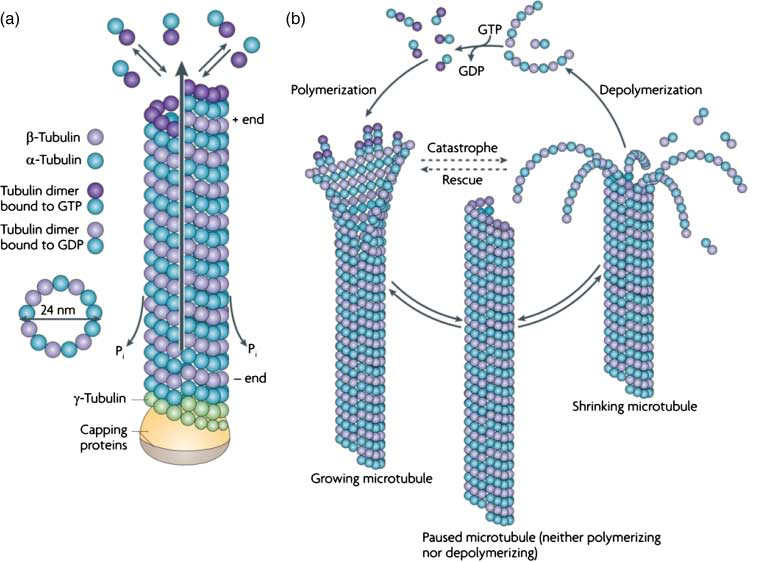
\includegraphics[scale=0.5]{Microtubule.png}
\caption{Construction et destruction des microtubules. }
\end{figure}
La tubuline, composée de deux sous-unité (alpha et bêta), s'associe en protofilaments de treize monomères, qui vont s'associer pour former de longs filaments creux de diamètre 25nm. Ces filaments sont polarisés, une extrémité ne comportant que des sous-unités beta ( notée +) et l'autre que des alpha (notée - ), la polymérisation ayant lieu à l'extrémité + et la dépolymérisation à l'extrémité -. 
Le microtubule est le filament le plus rigide du cytosquelette, sa longueur de persistance est de l'ordre du millimètre, bien plus que la taille d'une cellule. 

Dans les cellules eucaryotes, microtubules sont organisés autour d'un élément central : le centrosome. A partir de cet élément central, les microtubules irradient vers la périphérie cellulaire. 
Sur les microtubules, deux types de moteurs moléculaires se déplacent, les dynéines et les kinésines, respectivement de l'extrémité + vers - et de - vers +.  

Les microtubules organisent les éléments de la cellule et assurent le transport entre les organites, en particulier par le déplacement des vésicules. Les moteurs moléculaires conduisent les vésicules d'un organite à l'autre, par exemple les protéines nouvellement synthétisées vers l'appareil de Golgi, ou les protéines de la matrice extra-cellulaire vers la membrane. 

Les microtubules jouent un rôle prépondérant lors de la mitose. Ils s'assemblent en un fuseau au bout duquel se trouve les centrosomes. Au centre s'alignent les paires de chromosomes, qui sont séparés et emmenés vers les centrosomes. La plupart des drogues perturbant les microtubules bloquent la mitose et sont utilisées pour cette raison dans les traitements anti-cancéreux. 

Par ailleurs, les flagelles et les cils, par exemple le flagelle du spermatozoïde, sont composés d'un faisceau de microtubules animé par les moteurs moléculaires. 

\subsubsection{Filaments intermédiaires}

Contrairement à l'actine et à la tubuline, qui sont conservées et exprimées dans tous les types cellulaires, les filaments intermédiaires sont une famille de protéines dont l'expression dépend du type cellulaire (à l'exception de la lamine). 
Leur assemblage ne nécessite pas non plus l'hydrolyse d'ATP ou de GTP, il est spontané, et il n'existe pas de moteurs moléculaires se déplaçant sur ces filaments. 

Les réseaux de filaments intermédiaires sont liés aux protéines transmembranaires (cadhérines, intégrines) au niveau de structures appelées desmosomes (nom qui vient de la desmine) qui participent à l'intégrité mécanique des tissus. 

Le réseau de filaments intermédiaires est plus stable que les deux autres réseaux du cytosquelette, qui sont en construction et destruction permanentes. Leur rôle est principalement d'ancrer les différents organites dans la cellule. 

Les plus connus des filaments intermédiaires sont sans doute les kératines, exprimées dans les cellules épithéliales et qui sont le constituant principal des poils et des ongles des mammifères (la kératine des reptiles et des oiseaux ne présente pas d'homologie avec celle des mammifères). 

La vimentine est exprimée dans toutes les cellules d'origine mésenchymateuse. Elle joue un rôle dans la localisation des vésicules bien que ne participant pas directement à leur transport : le réseau de vimentine interagit avec celui des microtubules. Elle est également impliquée dans la régulation de l'adhésion et de la migration cellulaire. 
L'expression de vimentine est souvent un marqueur de la transition épitéhlio-mésenchymateuse. 

Plusieurs types de filaments intermédiaires sont exprimés dans les neurones, et deux types sont spécifiquement responsables de la transparence du cristallin. 

\subsubsection{Les lamines}
\begin{figure}
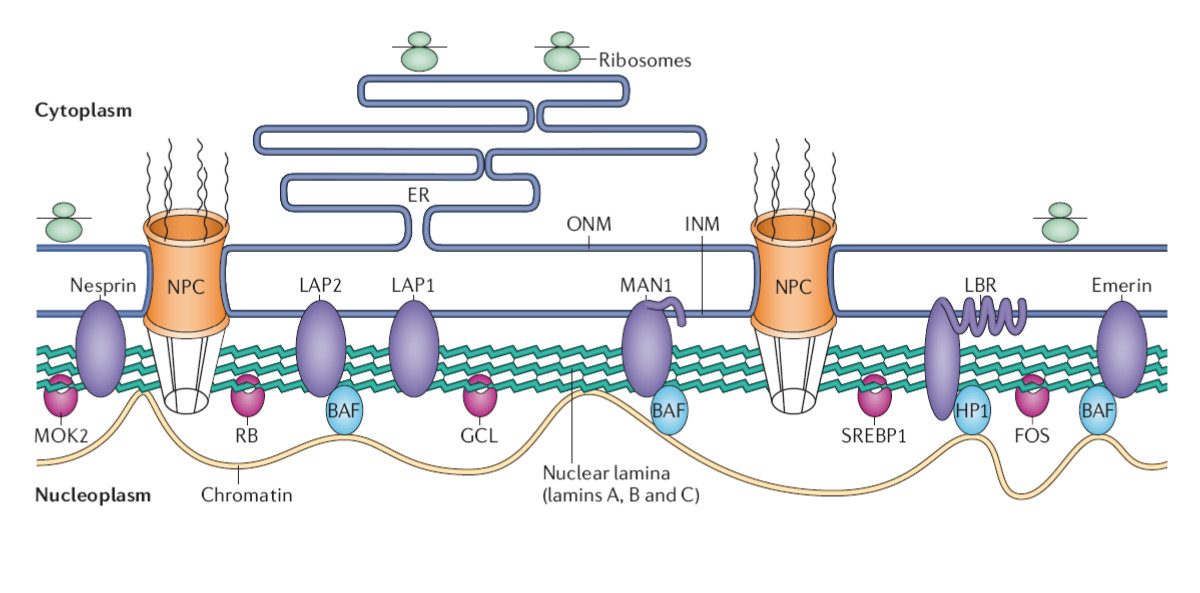
\includegraphics[scale=1.5]{Structure_and_function_of_the_nuclear_lamina.jpg}
\caption{Les lamines soutiennent l'organisation de la membrane nucléaire. Illustration par  \cite{coutinho}}
\end{figure}
Les lamines diffèrent des autres filaments intermédiaires sur plusieurs points. Elles ne forment pas un réseau dans toute la cellule mais sont localisées à la membrane nucléaire, et elles sont exprimées dans tous les types cellulaires. 

Les lamines forment un réseau soutenant la membrane nucléaire interne, dans lequel sont ancrés les pores nucléaires. Par l'intermédiaire de protéines comme la nesprine, le réseau laminaire est couplé mécaniquement au cytosquelette d'actine de la cellule et il est couplé à l'actine nucléaire par l'émerine, protéine qui coiffe la pointe des filaments d'actine et augmente leur polymérisation. 
Le réseau de lamines est nécessaire au maintien de l'intégrité du noyau et définit ses propriétés mécaniques. 
Les lamines organisent également la chromatine à l'intérieur du noyau et contribuent à réguler l'expression du génome (\cite{dechat_2008}).

La progéria est liée à des mutations sur le gène de la lamine A  et le syndrôme de dystrophie musculaire d'Emery-Dreifussà des mutations de l'émerine. 


\subsubsection{Filaments intermédiaires dans les cellules musculaires}
\begin{figure}
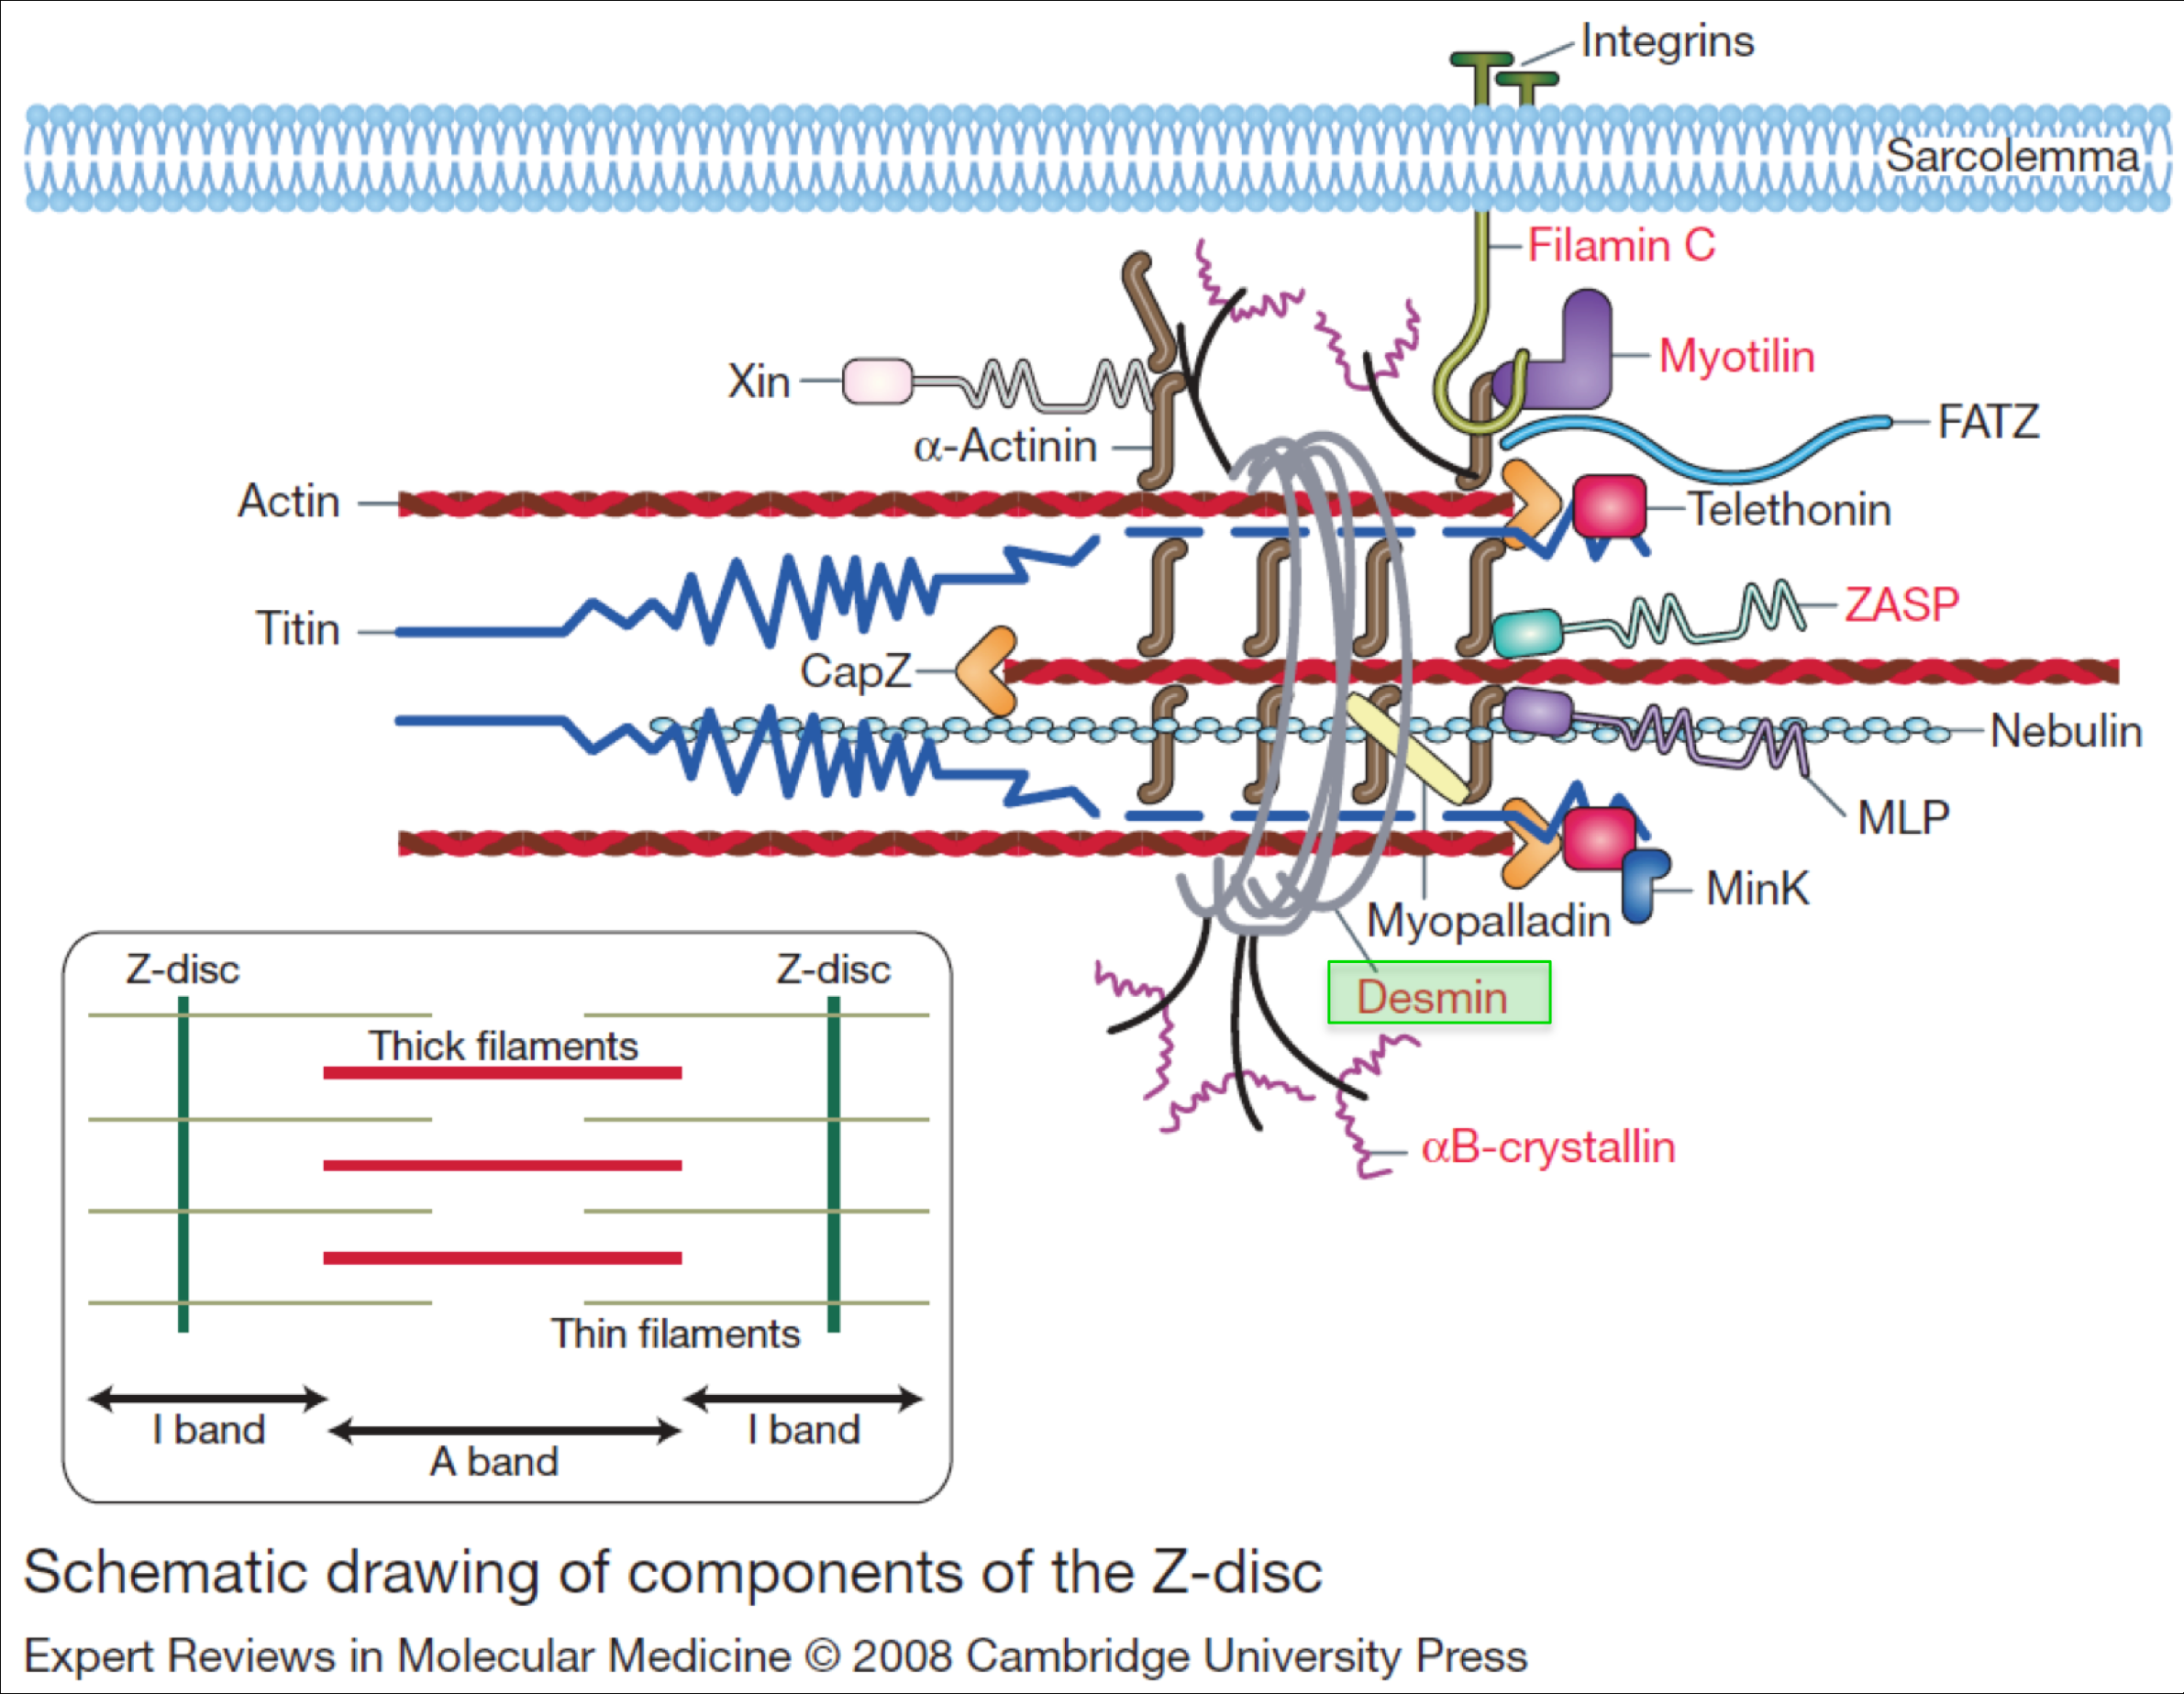
\includegraphics[scale=0.15]{sarcomere.png}
\caption{Rôle de la desmine dans l'organisation des fibres musculaires.}
\end{figure}
Quatre types de filaments intermédiaires sont exprimés dans la cellule musculaire : la desmine, la vimentine, la lamine et la synésine. 
La desmine et la vimentine ont des structures suffisamment proches pour pouvoir former des hétéro-dimères et s'associer dans des filaments. La synésine ne peut former que des hétéro-dimères avec les autres filaments intermédiaires. 

La desmine, la vimentine et la synésine ont un rôle dans l'organisation des fibres musculaires qui sera développé dans le chapitre consacré au muscle. 



\subsubsection{Actine}
  
L'actine constitue le réseau du cytosquelette le plus versatile et le plus dynamique. Son réseau est constamment réorganisé, et elle est le composant essentiel de la motilité cellulaire. 

Toutes les cellules eucaryotes expriment des actines, qui sont hautement conservées de la levure jusqu'à l'humain. Ce sont également des protéines très exprimées, et l'actine peut représenter jusqu'à 15\% de la masse de protéines dans une cellule \cite{Molecular Biology of the cell 4th edition}.

La membrane plasmique est une bicouche lipide qui a de faibles modules élastiques. Un réseau dense et très branché d'actine forme une couche rigide sous la membrane et confère sa forme à la cellule : le cortex d'actine. Ses propriétés sont essentielles dans les déformations des cellules et dans l'interaction de celles-ci avec un subtrat. 
Dans le volume de la cellule, l'actine forme un réseau moins dense. \textit{In vitro} on peut observer des faisceaux de filaments appelés fibres de stress. 
Dans le muscle, l'actine et ses moteurs associés (les myosines) forment une organisation spécialisée responsable de la contraction musculaire, appelée sarcomère, qui sera décrite dans le chapitre dédié au muscle.

L'actine interagit avec un très grand nombre de protéines, ce qui confère au réseau un caractère particulièrement dynamique. L'actine n'est pas limitée à un rôle mécanique, elle a également des rôles de régulation de l'expression du génome et d'organisation de l'ADN. 

Le couplage entre le rôle mécanique de l'actine et son rôle transcriptionnel est au c\oe ur de ce travail de thèse, c'est pourquoi l'actine sera présentée en détail dans un chapitre dédié. 




\section{Expression du génome}

Le génome d'un organisme contient toute l'information nécessaire à la reconstitution de l'organisme entier. Cependant, il est évident dans un organisme pluricellulaire que si toutes les cellules contiennent le même génome, elles ne l'expriment pas de la même manière. C'est également le cas chez des être unicellulaires : des bactéries ou des levures ayant le même génome ne vont pas l'exprimer de la même manière selon les conditions extérieures. 

Les parties codant directement pour des protéines ne représentent qu'une toute petite partie de l'ADN. Autour des séquences codantes, le reste du génome permet de déterminer quelles protéines doivent être synthétisées, et dans quelles quantités. 

\subsection{Des gènes aux protéines}

Le chemin d'un gène à une protéine fonctionnelle passe par trois étapes principale : la transcription de l'ADN en ARN, la maturation de l'ARN et la traduction de l'ARN en protéine 

\subsubsection{La transcription}

L'information génétique est stockée dans l'ADN, pour y être protégée et transmise d'une génération à l'autre. Les quatre bases de l'ADN fonctionnent par paires, et grâce à ce mécanisme un brin d'ADN peut être complété par sa séquence miroir. 

Lorsque toutes les conditions d'expression sont réunies, l'ARN polymérase peut se fixer sur l'ADN au site de début de transcription. Le complexe ouvre l'ADN, et permet aux bases de l'ARN, Adénine, Uracile, Guanine et Cytosine, de compléter les bases de l'ADN, respectivement Thymosine, Adénine, Cytosine et Guanine. L'ARN polymérase progresse ainsi jusqu'à rencontrer une séquence terminateur sur l'ADN. 

À l'issue de cette étape, un ARN a été transcrit directement à partir de la séquence codante. 

\subsubsection{La maturation de l'ARN}

Après sa transcription, l'ARN subit plusieurs transformations. Des éléments sont ajoutés à ses deux extrémités, pour assurer sa stabilité et sa reconnaissance par les ribosomes. 
L'ARN transcrit comprend deux types de séquences, les introns et les exons. Seuls les exons contiennent l'information des acides aminés pour coder la protéine. 
L'ARN va subir une étape d'épissage : les introns sont retirés de l'ARN jusqu'à ce qu'il ne reste que l'enchaînement des exons. Lors de cette étape, tous les exons peuvent être réassemblés, ou seulement une partie d'entre eux. Les protéines synthétisées par ces reconstitutions différentes seront différentes : on parle d'épissage alternatif. 
Un même gène peut donc coder pour des protéines différentes grâce au jeu de l'épissage. Par exemple, il existe chez la drosophile, un unique gène peut coder pour plus de 38 000 protéines différentes \cite{schmucker}, ce qui est du même ordre de grandeur que le nombre total de gène dans le génome de la drosophile. 

Après sa maturation, l'ARN messager est exporté du noyau pour se diriger vers le réticulum endoplasmique.

Tous les ARN n'ont pas vocation à être traduits en protéines : certains vont accomplir leur fonction sous cette forme. C'est le cas des éléments de la machine de traduction (ARN de transfert et ARN du ribosome), ou des micro-ARN, qui vont participer à la régulation de l'expression des gènes en aval de la transcription.

\subsubsection{La traduction}

Le code génétique est la correspondance entre des triplets de nucléotides et les acides aminés qui composent les protéines. 

La traduction commence au codon start le plus proche du début de l'ARN messager. La plupart du temps, chez les eucaryotes, il s'agit d'un triplet AUG, codant pour une Méthionine, cependant on découvre de plus en plus de séquences qui commencent avec un codon start alternatif. C'est le cas par exemple de la protéine Myocardin-Related Transcription Factor A, qui a deux variants d'épissage, l'un débutant par un codon GTG (Valine) \ref{scharenberg_2014}

Le travail de traduction est assuré par le ribosome, un assemblage complexe de protéines et d'ARN et par des ARN de transfert. Les ARN de transferts sont l'assemblage d'un ARN replié en croix et d'un acide aminé. À une extrémité, l'ARN présente un triplet anti-codon, le complémentaire d'un codon du code génétique. À l'autre se trouve l'acide-aminé correspondant à ce codon. 

Au début de la traduction, le ribosome se fixe sur le codon start, puis, il va chercher un ARN de transfert dont le triplet anti-codon corresponde au premier triplet sur la séquence à traduire. Comme quelqu'un qui teste différentes clés pour ouvrir une serrure, le ribosome va chercher l'ARN de transfert qui lui permet de faire correspondre un acide aminé à un codon. Lorsqu'il l'a trouvé, il attache l'acide aminé au précédent de la séquence, et ainsi de suite jusqu'à arriver à un codon stop. 

On parle souvent \emph{du} code génétique, car il est commun à un grand nombre d'êtres vivants, mais il en existe des variantes apparues au cours de l'évolution. En particulier, dans les cellules eucaryotes, l'ADN des mitochondries utilise un autre code génétique que celui de l'ADN de la cellule elle-même. 

\subsubsection{Modifications post-traductionnelles}

Les protéines commencent à se replier dès le début de leur synthèse par le ribosome. Mais certaines requièrent l'aide d'autres protéines, appelées chaperons, pour arriver au repliement correct. D'autres encore nécessitent des modifications chimiques après la traduction. 

Tous les acides aminés peuvent faire l'objet de modifications post-tranductionnelles. La plus connue est sans doute la phosphorylation, ajout d'un groupe phosphate à un acide aminé par des enzymes, les kinases. La phosphorylation joue le rôle de bouton on/off pour un grand nombre de protéines dans des voies de signalisation. Ce sera le cas des voies de signalisation qui seront présentées au chapitre 3, faisant intervenir les kinases ROCK, LIMK ou ERK1/2. 
Autre exemple de modifications, l'oxydation de l'actine sera également évoquée au chapitre 2. 


\subsection{Régulation de l'expression du génome}

\subsubsection{Réorganisation de la chromatine}

L'ADN est stocké dans la cellule sous une forme condensée, la chromatine. Il est enroulé autour de complexes de protéines appelées les histones. Selon leur état biochimique (acétylation, méthylation) les histones forment un enroulement plus ou moins compact de l'ADN. Par exemple, chez les femelles mammifères, l'un des deux chromosomes X est désactivé afin de ne pas avoir deux fois plus de transcription des gènes portés par ce chromosome qu'un organisme mâle. Il est condensé définitivement sous forme d'hétérochromatine. 

La compaction de l'ADN dans l'hétérochromatine ou dans l'euchromatine détermine donc quels gènes sont accessibles pour être transcrits et quels gènes sont désactivés dans l'hétérochromatine. 
La régulation de cette organisation par la modification chimique des histones est donc la première étape de la régulation transcriptionnelle du génome. 

\subsubsection{Les facteurs de transcription}

L'ARN polymérase ne peut pas se lier seule de manière stable sur l'ADN pour initier la transcription. 
Les facteurs de transcription forment une famille de protéines qui ont pour rôle de se fixer sur l'ADN en amont de la séquence à transcrire pour contribuer à l'expression du gène ou au contraire pour la réprimer. 

Un facteur de transcription reconnaît une séquence spécifique sur l'ADN en amont du gène régulé, le promoteur. Les promoteurs en amont d'un gène vont déterminer quels facteurs de transcription vont être capables d'activer la transcription. Des gènes partageant le même promoteur vont être activés par les mêmes facteurs de transcription et répondre aux mêmes stimuli.  

Dans le développement des êtres pluricellulaires, la différenciation des cellules souches totipotentes de l'embryon en différents types de tissus va être orchestrée par l'activation de nombreux facteurs de transcription. 

Les facteurs de transcription vont également être impliqués dans les réponses d'une cellule ou d'un organisme à des signaux biochimiques (hormones, facteurs de croissances, inflammation, poisons, toxines \dots) provenant de cellules voisines (par l'intermédiaire des liaisons transmembranaires entre deux cellules, par une structure spécialisée comme une synapse ou sécrété dans le milieu extra-cellulaire par les cellules voisines) ou des tissus éloignés (hormones circulant dans le corps), mais aussi à des signaux environnementaux comme la température, le choc osmotique, les contraintes mécaniques, l'exposition à la lumière du soleil  \dots

Les facteurs de transcriptions se lient directement à l'ADN, ils doivent donc être présents dans le noyau pour accomplir leur fonction. Certains facteurs de transcriptions sont ainsi régulés par leur localisation : lorsqu'ils sont confinés hors du noyau, ils ne peuvent pas être actifs. C'est le cas du récepteurs des \oe{}strogènes, qui est présent dans le cytoplasme en l'absence d'hormones et va être transporté dans le noyau lorsqu'il sera lié aux \oe{}strogènes.

Un facteur de transcription peut recruter d'autres protéines, comme des coactivateurs (ou des corépresseurs) qui vont l'amplifier (ou diminuer) l'activation de la transcription. Ces cofacteurs peuvent alors eux-même réguler l'activité transcriptionnelle par leur activité ( en particulier leur état de phosphorylation) ou par leur localisation. C'est le cas du mécanisme de régulation de Serum Response Factor, qui sera détaillé dans le chapitre 3. 

Un facteur de transcription peut également recruter des protéines qui vont changer localement l'état de compacité de la chromatine, afin de rendre le gène plus facilement ou plus difficilement accessible. 



%\end{document}